\chapterauthor{Jay Lofstead}{Sandia National Laboratories}
\chapterauthor{Eric Barton}{Intel}
\chapterauthor{Matthew Curry}{Sandia National Laboratories}
\chapterauthor{Carlos Maltzahn}{University of California, Santa Cruz}
\chapterauthor{Robert Ross}{Argonne National Laboratory}
\chapterauthor{Craig Ulmer}{Sandia National Laboratories}

\chapter{The Convergence of Enterprise, Internet Scale, and High Performance
             Computing Storage Infrastructures}

\section*{Abstract}
Large scale storage infrastructures have been significantly impacted by the
growth in data analytics applications. High Performance Computing storage
infrastructures, once the extreme end of the storage scale spectrum, must now
adapt to technologies optimized for large scale data analytics applications.
Hardware changes, such as storage class memory, are also affecting how
the exascale storage stack will be constructed. We examine use cases, trends,
convergent technologies, and new opportunities generated by this technology
blending.

\section{Introduction}\label{sec:intro}
HPC infrastructures have grown around the requirement to handle large,
decomposed data structures for parallel computation. Single data objects may be
hundreds of terabytes spread across an entire machine. Parallel storage systems
have grown trying to address performance and storage requirements while
maintaining backwards compatibility with the standard POSIX interface and
semantics.  Unfortunately, this is proving increasingly difficult, as the POSIX
specification was not designed to efficiently support parallel
storage~\cite{kimpe:2014:storagemodels}.

Big data and internet-scale applications, on the other hand, focus on searching
through immense volumes of small, loosely associated items looking for patterns
or correlations that may lead to insights. Some science applications, such as
genomics, have a workload pattern similar to these big data
applications. Parallel file systems are not well suited to these workloads
because the broad, relatively continuous read demand of independent items does
not benefit from the coordination overheads of parallel file systems. Instead,
distributing loosely coordinated storage across the compute infrastructure makes
more sense. With pressures to effectively leverage a single platform for these
disparate workloads and the shifting storage market, new considerations for how
to design storage resources for extreme scale compute systems must be made.

Traditionally, the HPC market has focused on supporting coherent and consistent
output methods from parallel sources to parallel targets. This requirement is
driven from validating that the output of a single item is complete and
correct. Largely, the workload is write-intensive during the expensive, at scale
computation process with a read-intensive phase lasting months on cheaper
machines or at small scale with low priority. File systems like the dominant
Lustre~\cite{braam:2002:lustre-arch} and GPFS~\cite{schmuck:2002:gpfs} systems
have been carefully optimized to address these workloads.

The big data market has opposite priorities. The big computation phase requires
reading large quantities of data for processing at scale. The output from this
process can be handled at much smaller scale later and is orders of magnitude
smaller. Given the read-dominant focus, the overhead inherent in coherent and
consistent storage for write intensive workloads is both unnecessary and a heavy
cost. Instead, systems like HDFS~\cite{shvachko:2010:hdfs} dominate.  These work
by storing files that will be read for processing throughout the compute area,
including the assumption that storage failures are common, prompting
replication.

The output from initial stream or file processing for the big data workloads use
distributed object-based storage technology. It offers independent,
uncoordinated data access with a simplistic key search space for subsequent
analysis. The profit potential for this market has caused an explosion in
specialized products aimed at accelerating this processing style.  For small
enough data sets, in memory object stores like memcached and Radius dominate.
For larger data sets, approaches like Google's Big Table are accomplishing the
same function. There are also hardware products targeting this market segment,
such as Kinetic~\cite{segate-kinetic}, offering a native object interface for
the devices connected directly to a network.

Adding complexity to this storage environment is the relentless performance
improvements and cost reductions for solid state storage, like NAND-based flash
memory. These devices have already rendered 15,000 RPM disk drives obsolete.
The 10,000 RPM disk drives will not survive for more than a few more years.
New disk technology like shingled drives~\cite{wood:2009:shingled-media} offer
a path for disks to survive longer. The enormous capacities for read intensive,
write infrequently workloads is very attractive for many communities. For
example, storing images created sequentially for later read-intensive
processing can yield a better cost/performance balance.

This chapter investigates these new technologies and how they affect extreme
scale computing. We evaluate how the HPC environment can and must adapt to this
new storage environment to address future computing needs and to take advantage
of the different kinds of technology being developed. We will also consider the
planned reintegration of large scale computing from the split of big data
applications from simulation-based computing with both the necessary and forced
integration of these large, expensive platforms for multi-use.

\section{Existing File Systems}

HDFS developed to support the Hadoop implementation of the MapReduce system. It
offers a distributed, replicated file store optimized to support the MapReduce
processing configuration. Ceph~\cite{weil:2006:ceph} also addresses this
distributed computing infrastructure, but with a different emphasis. It seeks
to offer scale out performance for objects across a storage infrastructure
with unreliable storage.  However, Ceph has historically had some fundamental
assumptions that incur overheads that are unacceptably large for a high end HPC
center~\cite{wang:2013:ceph}.  With the rise of cloud systems using
object-based storage, such as Amazon's S3, the interaction style offered by
Ceph has been adopted for similar workloads. Ceph's unreliable storage handling
works for both new storage additions as well as failures and recoveries without
interruption. Ceph offers a complete file system including metadata management
support as well as an object system for users.
GlusterFS~\cite{boyer:2012:glusterfs} focuses on providing a network attached
storage interface to storage distributed throughout a cluster.  Rather than
providing metadata services, GlusterFS relies on the underlying storage file
system for most basic capabilities, such as security.

Parallel file systems are optimized to support large files that must be spread
across multiple devices. For example, a 100~TB file cannot fit on any current
storage device and cannot be stored with any performance. Parallel file systems
solve this problem by using multiple devices spread across multiple servers
together as if they are a single device. Data is striped across devices, all of
which can be written to or read from simultaneously. This parallel access
offers aggregate performance enabling manipulating very large files with
reasonable performance. Because of these characteristics, parallel file systems
are deployed on most simulation intensive large scale compute systems to handle
the large single object output characteristic of these applications.  Lustre is
arguably the most popular parallel file system appearing on a majority of the
Top500 machines. IBM's GPFS is increasing in popularity as optimizations
focusing on addressing big data workloads are incorporated.
PVFS~\cite{ross:2006:pvfs} offers a rethinking of some of Lustre's earlier
limitations to give better scalability characteristics.

~\\\noindent\textbf{Discussion}\\
The different optimizations distributed vs. parallel file systems offer are at
the cost of supporting the other kind of workload. As was mentioned above,
parallel file systems aim to support very large objects and aggregate
simultaneous writing and reading for a single object across the array. For
workloads consisting of entirely small objects, this functionality and overhead
is a cost. Similarly, the inability of the distributed file systems to handle
arbitrarily large objects and massive parallel simultaneous access to a single
object make them unsuitable for simulation workloads.

For both workloads, a more flexible object-based interface are being
considered. This is discussed more below.

\section{Bridging Technologies}

While the shift to object stores pushes forward, we do have several pieces of
bridging tecnologies that may transition easily into the object storage
environment.

For efficient checkpoint/restart storage, two similar approaches are leveraging
the complex storage hierarchy to keep this rarely needed data out of the
storage array. Scalable Checkpoint Restart (SCR)~\cite{moody:2010:scr} and the
Fault Tolerant Interface for Hybrid Systems (FTI) ~\cite{bautista:2011:fti}
both use other in compute area resources to address checkpoint writing and
recovery performance. SCR focuses on hierarchical modeling while FTI focuses on
supporting hybrid compute like GPU-based systems.

Also working to bridge the gap are burst buffers. In short, burst buffers are
some generally non-volatile memory (NVM) somewhere within the compute area
intended for use as intermediate storage of some sort.  One of the first formal
burst buffer products is DataWarp from Cray. IBM also has a similar product to
be deployed on machines in 2016. The goal of these technologies is to offer a
high performance, but limited capacity storage area as a fast cache for the
parallel file system. Other uses for this storage is not the primary concern.
The motivating use case is that buying sufficient disks to achieve the
necessary parallel, aggregate performance is too costly, takes up too much
space, and has too many failures just to the very large number of devices.
Instead, disk is bought primarly for capacity while the burst buffer is bought
based on performance. The combination price yields less total storage, but the
performance characteristics are more favorable. Moving to a pure NVM solution
directly is too cost prohibitive for the next several years. Capacity and
durability are still too expensive.

\section{Object-Based Stores}\label{sec:intro}

The earliest object store is probably the Wisconsin Storage
System~\cite{1985:chou:wisconsin-storage} published in 1985. It offered a
general storage infrastructure for both databases and file systems. Many
current systems were built using a similar infrastructure, such as
Lustre~\cite{braam:2002:lustre-arch}, GPFS~\cite{schmuck:2002:gpfs}, and
Panasas~\cite{welch:2008:panasas}. The general idea is to offer s a
standardized way to address an arbitrary storage space with a key-based access.
These object storage systems assume that some sort of structure is imposed on
top to track what objects correspond to which user items.

While object storage may have been used behind the scenes for years, raw
object storage exposed to the end-user programmer did not into vogue until the
big data era arrived. System developers for big data processing realized that
the overhead imposed by the object management forced serialized or at least
coordinated access. By shifting the mapping load to the end-user programmer
level and using the object storage layer directly, greater perceived
performance can be achieved. In many cases, by stripping down the requirements
to the absolute minimum required semantics for a particular application,
actual performance gains are achieved. The explosion of specialized storage
systems like HDFS and GFS represent this model. Key for this model achieving
performance is the ability of each process to work independently without any
required consistency or coherence with neighbor processes potentially working
on part of the same data set. The dominant object stores are systems like
Memcached~\cite{fitzpatrick:2004:memcached}. This stands in stark contrast to
how supercomputing applications generally operate.

The supercomputing domain maintained the consistency requirements due to the
bulk synchronous parallel processing. Instead, parallel, that is coordinated,
file systems were embraced. The challenge today is that parallel file systems
are having difficulty effectively scaling to handle the IO demands.

Here we want to talk about how object-based key-value stores are used for big
data applications summarizing the specific features that identify this market
segment.

\subsection{HPC Oriented Object Stores}

Parallel file systems inherently have an object-like layer beneath the surface.
The requirement to spread a single file across multiple devices for capacity
reasons alone prompts this approach. The actual implementation may vary, such
as using individual files within a local file system, each representing part
of parallel file. Popular examples include
Lustre~\cite{braam:2002:lustre-arch} and GPFS~\cite{schmuck:2002:gpfs}.

In some cases, directly using a key-value store for HPC applications is being
considered~\cite{yin:2014:key-value-parallel}. The next generation Lustre
project is also considering a key-value infrastructure~\cite{barton:2013:lustre}
to address performance challenges.

The real challenge with key-value stores for HPC applications is the metadata
management. All of these projects have taken a similar step to the big data
application is that the applications are required to manage the object list to
determine what data is stored in which object.

\section{Next Generation HPC Storage Systems}\label{sec:intro}

Next generation storage infrastructures are taking on several different forms
with additional approaches both possible and likely. Almost certianly, multiple
of these approaches will last including evolutions of existing systems such
as IBM's GPFS. This section discusses four examples of different kinds of
storage infrastructures for the exascale environment.

\subsection{Lustre/DAOS}

The US Department of Energy is using a ``Fast Forward'' series of projects to
kickstart needed developments in the vendor space. One such project is the
Storage and I/O (FFSIO). The basis for this is extending the existing Lustre
infrastructure to offer an object interface, incorporate support for burst
buffer-like technoligies, and demonstrate use through a client I/O library. 
The first phase completed in 2014 and the second phase started in late 2015.

\begin{figure}[htbp]
\vspace{-0.10in}
\centering
\includegraphics[width=\columnwidth]{chapters/chapter1/figures/arch-mapping}
\vspace{-0.15in}
\caption{FFSIO Architecture and Component Mapping}
\label{fig:arch-mapping}
\vspace{-0.15in}
\end{figure}

Overall, the system design (see Figure~\ref{fig:arch-mapping}) consists of a
friendly end-user API that manipulates either the I/O Dispatcher layer or the
DAOS (Distributed Asynchronous Object Storage) layer.

The first phase design focuses on a few themes. First, a container and object
structure is assume. Second, transactions are integral to offering decoupled
performance. And third, hide additional API complexity behind a friendly
end-user API.

\subsubsection{Containers and Objects}
FFSIO presents a object-like interface that is mostly backwards compatible with
the standard POSIX files that an end-user API like HDF5 would create. It has
containers that represent files and objects of different types to represent
the different kinds of data stored for a ``file''. To keep a pure view on the
system, there is no master container or any other such construct. Instead, it 
is assumed that a user or system will specify a standard well-known container
that contains a list of available other containers. Some additional complexity
is introduced through this approach, but the decoupled requirement to update a
central metadata service for any file creation or access operation is
eliminated. Instead, either the user or policy would have to keep track of
available containers. The reasoning behind this structure is a bit complicated,
but quite reasonable.

Potentially extreme overheads for writing logically contiguously formatted data
is well documented. For example, ParColl~\cite{yu:2008:parcoll} showed as much
as 90\% overhead on as few as 512 processes. For the Six Degrees of Scientific
Data~\cite{lofstead:2011:six-degrees} work, the authors were unable to perform
some performance comparisons because a single data output could not be written
in the maximum normal job time. These sorts of impacts are prompting rethinking
the logically contiguous format favored by popular APIs like HDF5 and PnetCDF.
The perceived advantages when these formats were selected have not proven to
scale to very large, 3-D domain decompositions in particular. DAOS, offers the
object storage infrastructure while the HDF5 API at the end-user level is
maintained almost exactly. The only end-user API changes are related to
incorporating transactions. This shift almost exactly maintains backwards
compatibility while taking advantage of more scalable infrastructures.

\subsubsection{Transactions}
The system jitter and other causes for processes to fade out of sync affect
overall I/O performance as well. While transactions are typically seen as a
synchronous operation that blocks while all participants manage state, FFSIO
takes a passive approach and manages transactions asynchronously. The key idea
is to keep writes in a log-style copy-on-write structure and annotate each
write with which transaction it is part of. An overall transaction mapping
knows how many writes are expected and can decide when a transaction is
complete or not. By monitoring the system status, it can passively detect many
failures abort the affected transactions. The potential overheads to this
approach are refining the idea, but the core concept shall remain the same.

Transactions are manifest in two different ways. First, the end-user API layer
can opt to have the FFSIO system manage the transactions by that layer
tracking the status of all clients directly. Second, transactions can be
managed by the end-user layer themselves with a single process indicating the
transaction state to the FFSIO layer. The idea for the former approach is that
it offers transactional functionality without undue end user code changes. At
the IOD and DAOS layer, transactions are handled slightly differently.

The IOD layer is intended as a staging area for data that may or may not need
to be written to persistent storage. This is one implementation of the burst
buffer concept. The key idea is that the transactions in this layer may or may
not ever be pushed down to the DAOS layer. Instead, once the data set is
processed, only the analyzed results will be saved eliminating the need to
write large, temporary data sets to the slower, but much larger capacity
storage array. However, these transactions are connected to those at the DAOS
layer.

The DAOS layer is intended to function as a general object store that would
replace an existing data center wide shared parallel file system. Anything
written to this layer is expected to have longer lifetimes and potentially be
accessible from other platforms. Since the transactions work a bit differently,
in particular some sequential transactions may be missing, the name is changed
to epochs instead. The slightly different idea for an epoch is to represent
some important saved state. Since it is likely a revision of an existing
version, differencing mechanisms are tested to determine how to efficiently
store both versions with less space and minimal reconstruction overhead. When
small changes are persisted, the space savings can be enormous.

The Doubly Distributed Transactions Project ({D\textsuperscript{2}T}) offers a
more general approach to
transactions~\cite{lofstead:2012:txn,lofstead:2014:txn}. The end-user
programming cost is higher to support the more general use. Other than the
synchronous requirement for failure detection, the performance is excellent.

For future transactional use in the storage hierarchy, some mixture of the
three approaches is likely. The passive transactions will be used for backwards
compatibility. The end-user, single process managed transactions will work well
for storage system interactions. The {D\textsuperscript{2}T} approach could be used in isolation or
to support the end-user, single process managed transactions.

\subsubsection{API Complexity}
One of the complexities of the FFSIO stack is addressing various scale
platforms. For the largest platforms, including an IOD layer makes sense. The
particular architecture may vary, but that kind of technology will be important
to reduce compute throughput due to waiting for I/O to complete. For smaller
platforms, either the IOD layer is deemed unnecessary or it may be an extra
expense that offers little advantage. In this case, omitting this component
both simplifies the system and offers more direct performance.

The challenge with this approach is that the end-user level must address both
the IOD and DAOS APIs directly and be able to choose for fully portable code.
The advantages of being able to effectively scale down were maintained by using
a higher-level end-user API, like HDF5. For such a professionally produced
library, offering a second version is not a major undertaking. Further, it
enhances the HDF5 value by offering greater platform scalability.

\subsubsection{Discussion}
Overall, the shift from a traditional parallel file system to something like
the FFSIO system will be a big step forward towards supporting more big data
style hardware directly. While the design is not perfect, the second phase is
addressing most, if not all, of the detected shortcomings. 

\subsection{Kelpie/Data Warehousing}

Kelpie is a distributed, in-memory object store from Sandia National
Laboratories that serves as a building block in high-performance computing for
implementing custom, data-management services. The fundamental goal of Kelpie
is to provide a way for users to decompose their complex datasets into data
objects that the library can move between nodes in a safe but efficient manner.
Kelpie provides simple abstractions for dealing with distributed data, and
utilizes the Nessie communication library to orchestrate how data migrates
between nodes. Nessie provides (1) a low-level RDMA layer that has been ported
to different HPC fabrics and (2) an RPC layer that enables users to invoke
function calls and initiate RDMA transfers on remote nodes. Kelpie uses the
former to make an application's data objects accessible by the network
interface, and the latter to cooridinate data handoffs between nodes.

Kelpie manages data objects for applications, where a data object is a simply a
contiguous block of application data that is labeled with a globally-unique
key. The contiguous constraint is necessary because Kelpie registers the memory
with the network interface, which in turn allows the hardware to RDMA the data
without involving the kernel in virtual to physical address translation. The
key used to label an object has three components: an application-specific
identifier and a two-dimensional user label. The application-specific
identifier enables higher-level services to house different datasets in Kelpie
with isolation. Users are not required to use the second dimension of the user
label portion of the key. However, the second dimension is often useful for
grouping related items together in the store. For example when storing complex
mesh datasets in Kelpie, the first dimension of the key (or row) may be used to
describe a particular region of a mesh. The second dimension of the key can
therefore be used to organize different variables associated with the region
(e.g., node locations, pressure, or temperature). This approach allows each
variable's data to be stored in its own, independent block of contiguous
memory, and provides an opportunity for a user to easily downselect the items
they need when retrieving data from Kelpie.

Kelpie nodes are equipped with a Local Key/Value (LKV) structure for managing
data objects that are available in the local node. The LKV performs three
important tasks. First the LKV provides a means of tracking data objects that
are currently in transit and protect the system from deallocating an object
before remote nodes have finished transferring it. Second, the LKV structure
provides a means for data to be staged at a remote node with only trivial
involvement from the destination. For example, an application may push multiple
data objects to a node in anticipation of work that will be scheduled on the
remote node at a future time. Finally, the LKV structure provides a location
for applications to store callbacks to execute when data does arrive at a node.
These callbacks make the data store more active and are fundamental to
applications that are highly asynchronous or event driven.

In order to address scalability concerns, data management services for HPC
typically decompose their work in a hierarchical manner that maps owenership of
different portions of the dataset to different groups of nodes that are close
in proximity. Kelpie provides the ability to assemble multiple teams of nodes
together through a resource management interface. This interface allows users
to create and reference a team of nodes together to function as a single data
resource that employs a standard data API. A resource has three components: a
path-like name that allows a resource to be globally referenced and located by
the runtime, a list of physical nodes that implement the resource, and
client-side software that defines that policy for how data is managed in the
resource. Kelpie provides common implementations of resources, but is easily
extended with user-defined modules. A distributed hash table (DHT) is an
example of a commonly-used resource in Kelpie. A DHT is composed of N Kelpie
servers where data is distributed by using a hash of the first dimension of the
key to specify which node should store the object. The DHT resource client
software simply maintains the list of servers and then references the proper
destination when a user performs put or get operations. Users with reliability
concerns have made similar resources just by creating new client software that
stores a data object to the hashed server, and a replicated copy to its
neighbor. While resources may contain API extensions to support higher levels
of functionality, they all support basic communication primitives that enable
users to swap one type of resource in for another in most cases.

An example of how Kelpie is being utilized to support data management for
higher-level applications can be found in Sandia's DARMA project. DARMA is
developing an asynchronous, many-task (AMT) approach to computing that will
help codes scale to next-generation platforms. AMT codes specify their
execution in the form of a large, directed acyclic graph of tasks (or task DAG)
that can be scheduled by a runtime on distributed resources. The data objects
consumed and produced by each task form a dependency graph that dictate when
and where work can be scheduled. By utilizing Kelpie as the mechanism by which
data objects are migrated between different nodes and resources in the system,
DARMA can focus on the complex job of making policy decisions about how the
work should be orchestrated in the platform.

\subsubsection{Discussion}
Kelpie is clearly taking a different approach from the FFSIO project. By
pushing the key-value structure all the way up to the application, it requires
a whole new interaction between the applications and the storage
infrastructure, but at a potential advantage of much richer, higher
performance. For example, by integrating with the AMT management layer, Kelpie
can predictively move data as necessary or even guide the AMT manaagement layer
to place computation in a different location to avoid the data movement. Also,
by offering object level access beyond what an application would normally write
to storage, potentially new data access routines for richer analysis could be
integrated without requiring any application changes. Simply by registering all
data through Kelpie for use in the AMT management layer, other users could take
advantage of the metadata and select data for additional analysis without
worrying about explicit staging or writing to some persistent store.

\subsection{Hybrid Models}

A different take on the problem is being investigated in a DOE sponsored
project called SIRIUS primarily by Oak Ridge, Sandia, UC Santa Cruz, Rutgers,
and Brown. In this project, we seek to address the performance mismatch more
directly through several apporaches simultaneously.

First, using a single storage tier at a time leaves potential performance
untapped. Instead of the traditional structure where an output is pushed to a
particular storage tier and it is maintained on that tier (or partially through
some sort of hierarchal storage management system), all tiers are used directly
at the same time. For example, when writing a large data set for a molecular
dynamics code simulating crack formation, only certain areas contain important
features required for detailed analysis the rest of the data is not as
important. Consequently, SIRIUS seeks to write the important parts of the data
set to the fastest tier with the less important spooled to slower tier(s). In
many cases, if the output for the slower tier fails, the data set is still
usable enabling throwing away the less unteresting data set portions given
system performance pressures.

For performance reasons, much like the other solutions discussed above, SIRIUS
is assuming an object storage layer beneath the API. This layer could be DAOS,
Kelpie, the Sandia Sirocco storage system, Ceph, or any other object-based
infrastructures. Which object storage infrastructure employed will be flexible
depending on the data center and application workloads requirements.

Second, feature identification ane extraction can be expensive in time and
space or may not be applicable to the simulation type. For example, particle in
cell simulations use statistical measures for all particles in cell regions to
determine simulation values. Tagging particular particles as potentially
extraneous for a particular output is expensive. Instead, other techniques to
slice the data may be employed. For example, simple data rearrangement may
yield sufficient quality for most purposes dramatically reducing the data
volumes used in visualizations by a factor of more than 100x. By selecting
every fourth element in a mesh and then only selecting the 3 bytes required to
represent the sign, exponent, and the most significant bits of the mantissa is
a radical data reduction. This small data set version could be written to fast
storage while the other possible slicings can be written to slower storage
tiers that presumably have more capacity. By being able to slice data for
different placement and offering the signficiant data reductions with little
loss in analysis quality, time to insight can be improved. Should the full
quality data set ever be required, all of the pieces can be reassembled from
the various storage tiers and processed as a single unit. Alternatively, an
auditor offers a lossy approach.

Auditors are an idea that recognizes that while simulations have refined over
the years, much faster, simpler, older models can still be used over short
timeframes to get a very close approximation to the fine grained, fully
featured simulation. Using these older models as an auditor for the full
fidelity simulation, we can track, only over relatively short time and space
constraints, with radically less computational load and data sizes. By using an
auditor running along side the full fidelity simulation, the error magnitude
can be managed resetting the auditor when the drift is unacceptably large,
approximate data quality can be maintained. Using statistical techniques,
auditor output can be used to regenerate statistically similiar full fidelity
simulation values within a known error bounds forced by the state comparison to
determine the auditor drift. Using this approach major events or periodic
timesteps can be output using full fidelity while many intermediate results can
be output using the auditor state generating high quality lossy representations
of what the intermediate simulation state would be like. There are other lossy
approaches available. For example, ISABELA~\cite{lakshminarasimhan:2011:isabela} offers a sorted
data set with B-Spline curve fitting to reduce the data set size.
Delta~\cite{jeanbaptiste:2015:delta} looks at simple diffs to reduce the data set with low
space-time overheads with no loss. Wavelet compression~\cite{klappenecker:1995:wavelet} low
space-time overheads with potentially radially high data compression with
predictable error rates. Each of these approaches can be useful in different
circumstances.

Third, SIRIUS focuses on Quality of Service (QoS) to help guide users to
choosing an acceptable time/quality tradeoff for a given operation. For
example, in the data reoganization example above, using the every fourth point,
3 bytes of 8 bytes values may be able to be loaded and analyzed in 1 minutes.
Reading the full fidelity may take 2 hours. For a quick peak to see if the data
might be ``interesting'', the 1 minute overhead is likely enough. Should a
general feature seem to be present, a data set could be noted for later fully
detailed review. The 2 hour overhead could be scheduled rather than delaying
the interactive scientist.

\subsubsection{Discussion}
SIRIUS seeks to take advantage of the whole storage hierarchy to get maximum
I/O bandwidth. By incorporating technqiues to slice, compress, or lossy
compress the data, more efficient storage tier use can be achieved. Since only
the small, most important part of a data set is stored in the fast, small,
expensive tier, many more outputs or different applications can use the tier
without strong considerations about exhausting the capacity. By including QoS
measures as part of the system enabling users to interact with requests to
determine the quality/time tradeoff, end user productivity can be enhanced with
little to no loss of scientific validity. For final report and paper
submissions, the time can be spent for full fidelity data reads and analysis to
validate the results generated from the lower fidelity data versions. These
kinds of techniques will be increasingly important to maximize both platform
productivity as well as scientist productivity.

\subsection{Radical Departure}
The Sirocco Storage Sytem from Sandia takes inspiration from peer-to-peer
systems to rethink how a storage system should work for HPC. Instead of relying
on existing notions of striping files across storage devices, it is fully
object based and works under the idea of primarily caching under data
resiliency requirements.

Existing parallel file systems, such as Lustre, GPFS, Panasas, and
PVFS/OrangeFS, all offer a way to store objects larger than a single storage
device by striping data across devices simultaneously enhancing performance.
Each of these systems have optimized in a different way. Lustre exposes all of
the tuning parameters allowing users to tweak settings to optimize performance.
The downside is that these parameters must be managed to achieve good
performance. GPFS hides most of these parameters and attempts to manage
performance optimizations with moderate success. Panasas dynamically increases
the number of storage targets used for a file as the simultaneous parallel
writer count increases. PVFS/OrangeFS has optimize metadata operations reducing
the load on the metadata server.

Sirocco seeks to completely rethink this model to move away from the rigid
striping model with a separate metadata service into a storage fabric with an
inherent assumption that resources may be transient. This fundamental
rethinking is being done with a nod to backwards compatibility by offering a
POSIX interface that can access a particular view of the storage system. The
native interface is object based with containers collecting objects each of
which have multiple data forks that can be accessed through an address space.
These four abstract levels offers flexibility to address HPC, Experimental and
Oversational Data, and large scale data analytics needs.

The roots of Sirocco are in the Lightweight File Systems
(LWFS)~\cite{oldfield:2006:lwfs} project at Sandia from several years ago. LWFS
sought to strip down a file system to the bare, required components and allow
users to add additional capabilities paying the overhead for only those
features required. For example, the LWFS core consists of an object store with
authentication and authorization services only. Other features, such as naming
and consistency control, are left to separate services. Sirocco seeks to
provide the storage layer that an LWFS-style system would require. Keeping this
in mind will help explain some of the decisions made. For example, a
non-Sirocco client accessing or manipulating data is equivalent to going
directly to disk and reading or modifying bytes rather than going through the
file system interface. Protections against such access are not included since
it is intended to act like a device like disk only accessed through a file
system interface of some sort.

One way to think about how Sirocco works is as a reverse Bittorrent system. In
a typical Bittorrent system, a seed offers a file for others to replicate as
they request it. A tracker offers a directory to find where seeds are located
so that new clients can discover what is currently available. Over time, a
requested seed will be replicated to the local client based on pulling pieces
from a variety of sources currently offering a copy of the file. Which seeds
are available over time change dynamically making it likely that a new copy of
a file came from multiple sources, some of which were only available for part
of the transfer time.

Sirocco takes a reverse approach for writing because a client wants to store a
file into the server collection with some resilience properties. As it is
pushed into the space, it will be copied and replicated according to the device
characteristics and availability and resilience requirements asserted as the
data is pushed.

For reading operation, Sirocco will go find the current data version and return
it to the requesting user. For performance reasons, a user could force a copy
to migrate to a particular location. The old version may be flushed on a space
required and resilience considering basis. The collection of Sirocco servers is
referred to as a swarm further reinforcing the Bittorrent analog.

To understand how Sirocco works at a detailed level, several concepts and how
they work in Sirocco are required. Each of these are explored below.

\subsubsection{Logical Structure}
Logically, Sirocco uses a containers, objects, forks, and address spaces tuple to identify a particular byte. Each of these concepts plays a different role offering specific features.

All of these concepts rely on IDs or ranges. Each of these are represented by a 64-bit number. This specifies the size of all of these spaces. When considering these concepts, a rich format like HDF5 helps understand the purpose of each. Sirocco goes beyond HDF5's capabilities to offer new features common in other kinds of storage systems.

~\\\noindent\textbf{Containers}\\
The container is equivalent to a file in a traditional file system. The idea of
using a container rather than a file is that it is really a capability envelope
for an object collection rather than a single byte stream. Each container
contains zero or more objects.

~\\\noindent\textbf{Objects}\\
Each object can be though of as a variable in an HDF5 file. For example, an
array or scalar value may each be stored in a single object. The object 0 for
every container is reserved.

~\\\noindent\textbf{Forks and Address Spaces}\\
Each object can have multiple versions or views referred to as a ``fork''.
These forks are similar to the old Macintosh OS resource and data forks stored
for each file. In this case, the number of forks is limited by a 64-bit number.
The fork 0 for every object is reserved for information for the security
system. This highlights that forks can serve multiple purposes beyond simply
being a resource and a data fork for a file. In this case, there is a security
information fork. Another use would be to specify a compression level for a
version of data. If a particular compression type or level is available, it is
stored in a well known fork ID. This can also be used for versioning to offer a
rudimentary source control system or represent the old VAX VMS file versions
concept. Many other potential uses are also possible and not artificially
limited by the system.

To access data within a fork, a 64-bit address space is referenced. Each
selected address portion is called a {\em range}. When writing, data is provided
for the range and pushed into Sirocco. The address space is treated as a key
value store using the address ranges as the key and the data as the value. Each
value is versioned with the versions being accessible.

Each address space within a fork is limited to 4 GiB currently. For the short
term, users are required to write multiple ranges as part of an extent to write
a larger space.

\subsubsection{Storage Devices}
Storage devices are represented by a Sirocco interface. Each device has its own
Sirocco interface and has particular characteristics that determine how it is
used. For example, a RAM backing store may be used for a compute-node Sirocco
server or a disk may back a different Sirocco server. How and when these are
used is driven from the resilience characteristics requested for an extent.
Device collections that share the same characteristics can be thought of as
comprising a single storage tier. Sirocco makes no such association as it
treats all potential storage locations as peers and selects which to use based
on the resilience characteristics requested.

~\\\noindent\textbf{Device Characteristics}\\
Device characteristics affect two different system functions. First, they
specify the performance that can be expected when accessing the device. Second,
they specify a resilience metric that is used for data protection and
availability. Both of these work together to guide data placement and
migration.

The four basic characteristics are latency, bandwidth, load, and volatility.
The first two are exactly as expected for a storage system. Load is a dynamic
measure of how busy a storage device is currently. Migrating data to a heavily
loaded device is a poor performance choice if other options are available and
Sirocco considers this to try to offer the best overall performance. Volatility
is a measure of how safe data stored in this device is compared to other
devices. RAM vs. node local SSD vs. centralized SSD vs. disk vs. tape all offer
different volatility metrics. This metric in particular is used to implement
the resilience features.

When an extent is provided to the Sirocco API, two resilience characteristics
are provided--short term and long term. The short term requirement describes
how to store the data before the Sirocco API returns control to the user. For
example, if a two-copy on persistent store short term requirement is specified,
Sirocco will ensure that two storage devices meeting this requirement have
successfully acknowledged storing the data before returning control to the
user.

The long term resilience requirement comes into play as the amount of space
available is insufficient requiring data ejection or deletion. Any extent
selected for eviction or deletion will be reconciled according to the long term
resilience requirements. If the long term requirements specify resilience
characteristics typical of a tape system and insufficient additional replicas
to meet the resilience requirement exist, Sirocco will migrate the affected
data towards or into the tape system to free space required for the current
operation.

~\\\noindent\textbf{Finding Data}\\
Given the assumed transient device existence, Sirocco works to keep data with
required resilience characteristics as devices come and go. When a device is
discovered to be missing, any replicas stored on that device must find
alternative locations to preserve the required resilience. News of the missing
device is propagated to all participating storage servers so they can react to
the loss appropriately. When a new server comes online, a similar propagated
message informs the swarm of the new potential target and the characteristics
it offers.

Should all replicas for a file go offline effectively simultaneously, it is
possible for data to be stored securely, but not be accessible. Sirocco works
to minimize this possibility, but it is impossible to guarantee that data will
always be available unless all data is replicated on all storage devices--a
clearly infeasible solution.

~\\\noindent\textbf{Authoritative Copy}\\
Something that may come to mind with the broad discussion of having multiple
data copies for resilience and transient storage devices is how to know what
the ``official'' data version is. This is handled through the idea of an
authoritative data copy. By default, Sirocco selects one copy as the
authoritative copy. Should that copy be ``far'' from the client, the client can
request that the authoritative copy migrate to a nearby server to offer better
interactive performance.

~\\\noindent\textbf{Server to Server Communication}\\
Since Sirocco has no central point of control, any data can be requested or
written to any server in the swarm. If the data is not stored on that server,
Sirocco starts to search by asking nearby servers if they have or know where
the data is stored. As that message propagates out, the user will eventually be
told the data cannot be found or have the data returned to them. For a basic
request, the data may or may not migrate a copy to the server the client
initiated the request through. By requesting the authoritative copy migrate,
the user can force the primary copy to move to the server the request was
initiated through.

~\\\noindent\textbf{Client APIs}\\
While the native interaction for the 4-tuple (container ID, object ID, fork ID,
address space) is an object interface, it does not address needs of existing
applications or file system APIs. While this is the preferred interface since
it offers the richest interaction and control mechanisms, backwards
compatibility is required. A full POSIX interface has been implemented, but it
is limited. For example, a separate metadata service will be required for
naming that maps to containers. Also with this mapping, how to handle objects,
forks, addresses, and versions is required. By default, it serializes the
objects and forks, but only the most recent versions.

\subsubsection{Discussion}
The four simple 64-bit identifiers offers tremendous capacity and storage
system flexibility that should be able to address high end storage needs for
years to come. With these fixed numeric spaces, but no incorporated metadata
system, some operations are no longer apparent. For example, since all IDs exit
in theory and storage resources may come and go, the idea of ``creating'' or
``deleting'' something is alien. When a particular tuple is specified, as long
as the requester has authority to access that space, they will be given access.
When reading, if the requested space does not exist in the current space, a
``not found'' is returned. To delete an item, it must be cleared from the
system by doing a write setting the record length to zero.

Since performing since address space writes at a time may be highly
inefficient, the concept of a record and an extent exist. A record is the
version and length of a value that represents an address range within a fork.
An extent is a collection of records to be operated on. Most Sirocco APIs use
an extent rather than a record for data manipulation. Processing of extents is
in an undefined order and all have the same version. The extent processing is
done as a single transaction.

Sirocco fundamentally rethinks how to offer a storage system for a high end
computing environment. By rejecting the current zebra model for a peer-to-peer
style model, resilience features can be incorporated more easily. While some of
the limitations of this approach may complicate the file system interaction
built on top of Sirocco, the flexibility and features make considerations worth
the trouble.

\section{Conclusions}\label{sec:conclusion}

The growth in data analytics and the corresponding embracing of object-based
and key-value technologies is dramatically shifting the storage landscape. With
pressures to support both traditional HPC simulation workloads and large scale
data analytics on the same platforms, the pressures on HPC platforms, software
infrastructure, and applications continues to increase. Through adapting
programming models, such as using asynchronous many task with a system like
Kelpie to support data management, the changed storage features can be fully
exposed and embraced by the applications.

For existing applications that either cannot or will not shift to an AMT model,
systems like the FFSIO and SIRIUS offer alternatives that with only minimal
modification, the applications can achieve many benefits.

Based on our existing efforts and thoughts, the move to the distributed objects
and key-value stores will add complexity and incurr a loss from parallel file
system functionality. However, these costs are proving acceptable given the
performance and functionality gains being achieved. As the market and platforms
continue to shift, we see HPC applications being better able to take advantage
of data analytics infrastructure while the data analytics software will need to
make some adjustments to the different platform requirements for HPC
simulation-oriented machines. Eventually, both should be able to co-exist with
minimal performance loss. Ideally, both will benefit from the combination of
the best of both worlds.

\section*{Acknowledgements}
Sandia National Laboratories is a multi-program laboratory managed and operated
by Sandia Corporation, a wholly owned subsidiary of Lockheed Martin
Corporation, for the U.S. Department of Energy's National Nuclear Security
Administration under contract DE-AC04-94AL85000.

%\begin{figure}[htb]
%\begin{figure}[b!]
%\centerline{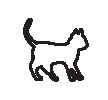
\includegraphics[width=150pt, height=150pt]{Chapters/chapter1/figures/cat.eps}}
%\caption[List of figure caption goes here]{Figure caption goes here. Figure caption goes here.}
%\end{figure}

%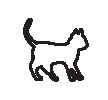
\includegraphics[width=\textwidth]{Chapters/chapter1/figures/cat.eps}
%\caption[Short figure caption]{Figure caption goes here.
%Figure caption goes here.
%Figure caption goes here.}
%\end{figure}

%\section{Glossary}
%\begin{Glossary}
%\item[Adaptable] An adaptable process is designed to maintain effectiveness and
%efficiency as requirements change. The process is deemed adaptable when there
%is agreement among suppliers, owners, and customers that the process will meet
%requirements throughout the strategic period.
%\end{Glossary}

